\documentclass{beamer}

\usepackage[utf8]{inputenc}
\usecolortheme{beaver}
\usepackage{caption}
\usepackage{subcaption}
\usepackage{mathtools}
\usepackage{todonotes}
\usepackage{amsmath}
\usepackage{bm}
\usepackage{listings}

\def\ci{\perp\!\!\!\!\!\perp}

\newtheorem{proposition}{Proposition}

\begin{document}

\title{A Simple Unified Approach to Testing High-Dimensional Conditional Independencies}
\author {Ankur Ankan \and Johannes Textor}
\institute{Radboud University}
\date{}
\maketitle

\begin{frame}
	\frametitle{Overview}
	\tableofcontents
	Motivation: How are CI tests used in causal inference.
	Background: Main types of CI tests with advantages/disadvantages.
\end{frame}

\section{Motivation}
\begin{frame}
	\frametitle{Motivation: Example DAG / Causal Bayesian Network}
	\begin{figure}
		\centering
		\includegraphics[scale=0.6]{imgs/example_dag.png}
		\caption*{An example of Directed Acyclic Graph (DAG) \footnotemark}
	\end{figure}
	\begin{center}
	DAGs imply CI: Each variable is conditionally independent of all non-descendants given its parents. E.g.

			$$ \text{\emph{XRay}} \ci \text{\emph{Pollution}} | \text{\emph{Cancer}} $$
			$$ \text{\emph{Breathing}} \ci \text{\emph{Smoker}} | \text{\emph{Cancer}} $$
	\end{center}
	\footnotetext[1]{\footnotesize{K. B. Korb, A. E. Nicholson. Bayesian Artificial Intelligence}}
\end{frame}

\begin{frame}[fragile]
	\frametitle{Motivation: Model Testing}
	\begin{itemize}
		\setlength\itemsep{1em}
		\item In applied research, most of the DAGs are made by hand
			based on domain knowledge.
		\item Important to test whether the model is consistent with the data.
		\item Conditional Independence (CI) tests can be used to verify model structure.
	\end{itemize}
	\vspace{1em}
	\begin{figure}
 	\begin{verbatim}
                              x2 df    p.value
 Brth _||_ Pllt | Cncr 4.7571803  2 0.09268115
 Brth _||_ Smkr | Cncr 9.0058063  2 0.01107679
 Brth _||_ XRay | Cncr 1.9104270  2 0.38472999
 	\end{verbatim}
		\caption*{Example model testing output from R package \emph{dagitty}}
	\end{figure}

\end{frame}

\begin{frame}
	\frametitle{Motivation: Structure Learning}
	\begin{itemize}
		\setlength\itemsep{1em}
		\item CI implies that no direct causal link exists between the variables. \newline
			$ \text{\emph{XRay}} \ci \text{\emph{Smoker}} | \text{\emph{Cancer}} \implies \text{No edge b/w \emph{XRay} and \emph{Smoker}} $

		\item Constraint-Based structure learning algorithms like PC
			and FCI use CI tests to systematically search for CIs
			in the dataset to determine model skeletons.
	\end{itemize}
	\begin{figure}
		\centering
		\includegraphics[scale=0.6]{imgs/example_sl.png}
		\caption*{Structure Learning Example}
	\end{figure}
\end{frame}

\section{Background}
\begin{frame}
	\frametitle{(Conditional) Independence}
	\begin{block}{Independence}
		Two random variables $ X $ and $ Y $ are independent,
		$ X \ci Y $ if and only if $ P(X, Y) = P(X) \cdot P(Y) $.
	\end{block}
	\vspace{1em}

	\begin{block}{Conditional Independence}
		Two random variables $ X $ and $ Y $ and are said to be
		conditionally independent given $ \bm{Z} $, $ X \ci Y | \bm{Z}
		$ if and only if for all $ z $ with $ p(z) > 0 $, $ P(X, Y |
		Z=z) = P(X | Z=z) \cdot P(Y | Z=z) $
	\end{block}
\end{frame}

\begin{frame}
	\frametitle{CI Testing is Difficult}
	\begin{figure}
		\centering
		\includegraphics[scale=0.7]{imgs/sl-adult-mi-crop.pdf}
		\caption*{Learned structure for US census income dataset using chi-square test}
	\end{figure}
	\begin{itemize}
		\item Testing for CI is much harder compared to testing for
			non-conditional independence.
		\item Especially in case of high cardinality or high number of
			conditional variables.
		\item In the continuous case, no test can exist which is calibrated and
			has power over all distributions where CI is True. \footnotemark
		\item Many different approaches and tests have been proposed.
	\end{itemize}

	\footnotetext[2]{\footnotesize{Shah, Rajen D., and Jonas Peters. "The hardness of conditional independence testing and the generalised covariance measure." The Annals of Statistics, 2020}}
\end{frame}

\begin{frame}
	\frametitle{Main classes of tests}
	\begin{itemize}
		\setlength\itemsep{1em}
		\item Stratification based tests
		\item Variable Importance based tests
		\item Residulaization based tests
	\end{itemize}
\end{frame}

\begin{frame}
	\frametitle{Stratification Based Tests}
	\begin{itemize}
		\setlength\itemsep{1em}
		\item Most common type for discrete variables. E.g. chi-square,
			mutual information based test etc. 
		\item Converts CI test into simple independence test by splitting 
			the dataset.
		$ D[X, Y, \bm{Z}] = \{ D[X, Y, \bm{Z}=\bm{z_1}], D[X, Y, \bm{Z}=\bm{z_2}], \cdots \} $	
		\item Runs test on each stratum and then combines the results.
	\end{itemize}
\end{frame}

\begin{frame}
	\frametitle{Statification Based Tests: Example}
	\begin{block}{}
	\begin{columns}
		\begin{column}{0.33 \textwidth}
			\begin{tabular}{c c c}
				X  & Y  & Z \\
				\hline
				X1 & Y1 & Z1 \\
				X1 & Y2 & Z2 \\
				X2 & Y1 & Z1 \\
				X3 & Y3 & Z2 \\
				\vdots & \vdots & \vdots \\
			\end{tabular}
		\end{column}
		\begin{column}{0.33 \textwidth}
			\begin{block}{}
				\begin{tabular}{c c c}
					X & Y & Z \\
					\hline
					X1 & Y1 & Z1 \\
					X2 & Y1 & Z1 \\
					\vdots & \vdots & \vdots \\
				\end{tabular}
			\end{block}
			\begin{block}{}
				\begin{tabular}{c c c}
					X & Y & Z \\
					\hline
					X1 & Y1 & Z1 \\
					X2 & Y1 & Z1 \\
					\vdots & \vdots & \vdots \\
				\end{tabular}
			\end{block}
		\end{column}
		\begin{column}{0.33 \textwidth}
			\begin{block}{}
				Test $X \ci Y$ in $ D_1 $.
			\end{block}
			\begin{block}{}
				Test $X \ci Y$ in $ D_2 $.
			\end{block}
		\end{column}
	\end{columns}
	\end{block}
	\begin{block}{}
		Combine the results
	\end{block}
\end{frame}

\begin{frame}
	\frametitle{Stratification Based Tests: Advantages/Disadvantages}
	\begin{itemize}
		\item As the number of conditional variables is increased, exponentially
			less data is available in each stratum.
		\item Looses power when number of conditonal variables
			are increased.
	\end{itemize}
\end{frame}

\begin{frame}
	\frametitle{Variable Importance Tests}
	\begin{itemize}
		\setlength\itemsep{1em}
		\item Based on comparing the probability models: $\hat{p}(x |
			y, z) $ and $ \hat{p}(x | z) $. E.g. Stochastic
			Complexity-Based Conditional Independence Test (SCCI) \footnotemark.
		\item If the simpler model doesn't fit significantly worse, implies $ X \ci Y | Z $.
		\item Can utilize any statistical model for which a reasonable goodness
			of fit exist.
	\end{itemize}
	\footnotetext[3]{\footnotesize Marx, Alexander, and Jilles Vreeken. "Testing conditional independence on discrete data using stochastic complexity." PMLR, 2019}

\end{frame}

\begin{frame}
	\frametitle{Variable Importance Tests: Example}
\end{frame}

\begin{frame}
	\frametitle{Variable Importance Tests: Advantages/Disadvantages}
	\begin{itemize}
		\item Can use any probabilistic model.
		\item Inherently asymmetrical. The result of $ X \ci Y | Z $
			can be different from $ Y \ci X | Z $.
	\end{itemize}

\end{frame}

\begin{frame}
	\frametitle{Residualization Based Tests}
	\begin{itemize}
		\setlength\itemsep{1em}
		\item Uses two estimators $ \mathbb{E}[X| Z] $ and $
			\mathbb{E}[Y | Z] $ and checks for the multiplicative
			association between the residuals. E.g.
			Partial Correlation test, generalized covariance measure etc.
		\item Relies on the theorem from Daudin [1980] \footnotemark 
			that under CI, if the estimators have ``valid'' residuals
			such that $ \mathbb{E}[R_{X|Z}] = \mathbb{E}[R_{Y|Z}] = 0 $,
			then $ \mathbb{E}[R_{X|Z} R_{Y|Z}] = 0 $.
	\end{itemize}
	\footnotetext[4]{\footnotesize Daudin, J. J. "Partial association measures and an application to qualitative regression." Biometrika, 1980}
\end{frame}

\begin{frame}
	\frametitle{Residualization Based Tests: Example}
	\begin{itemize}
		\item Train two estimators: $ E_1 = P(X | Z) $ and $ E_2 = P(Y | Z ) $.
		\item Use the estimators to do predictions for $ X $ and $ Y $. $ \hat{X} = E_1(Z) $, $ \hat{Y} = E_2(Z) $.
		\item Compute the residuals: $ R_X = X - \hat{X} $ and $ R_Y = Y - \hat{Y} $
		\item Test for $ Cor(R_X, R_Y) $.
	\end{itemize}
\end{frame}

\begin{frame}
	\frametitle{Residualization Based Tests: Advantages/Disadvantages}
	\begin{itemize}
		\item Any estimator can be used as long as it has ``valid'' residuals.
		\item There isn't an easy way to define residuals for oridanal or categorical variables. No residualization based test exists for categorical or ordinal variables.
	\end{itemize}
\end{frame}

\section{Proposed Method}
\begin{frame}
	\frametitle{Proposed Method}
	\begin{itemize}
		\setlength\itemsep{1em}
		\item Residualization based approach.
		\item Uses Li-Shepherd (LS) residuals \footnotemark. \todo[inline]{Partial copula?}
		\item Any unbiased estimator can be used. We show empirical results using Logistic Regression (GLM) and Random Forest (RFT).
	\end{itemize}
	\footnotetext[5]{\footnotesize C. Li and B. E. Shepherd. "A new residual for ordinal outcomes." Biometrika, 2012}
\end{frame}


\begin{frame}
	\frametitle{Residual for oridnal variables: LS-Residuals}
	Given an ordinal variable $ Y $ and an estimate $ \hat{p}(y) $ of $
	p(y) $, LS-Residual for sample $ y_i $ is defined as:
	$$ R_{y_i} = \hat{p}(Y < y_i) - \hat{p}(Y > y_i) $$
	\vspace{1em}

	For the binary case with $ Y \in \{0, 1\} $:
	$$ R_{y_i} = y_i - \hat{p}(Y = 1) $$
	\vspace{1em}

	For the conditional case for sample $ (y|z)_i $,
	$$ R_{y_i | z_i} = \hat{p}(Y < y_i | Z=z_i) - \hat{p}(Y>y_i|Z=z_i) $$

\end{frame}

\begin{frame}
	\frametitle{Residual for ordinal variables: LS-Residuals Example}
	\begin{columns}
		\begin{column}{0.5 \textwidth}
			$$ \hat{p}(Y) = \begin{array}{llll} Y_0 & Y_1 & Y_2 & Y_3 \\ 0.1 & 0.3 & 0.5 & 0.1 \end{array} $$
			$$ R_{Y_2} = \hat{p}(Y < Y_2) - \hat{p}(Y > Y_2) = 0.3 $$
			$$ R_{Y_3} = \hat{p}(Y < Y_3) - \hat{p}(Y > Y_3) = 0.9 $$
		\end{column}
		\begin{column}{0.5 \textwidth}
			$$ \hat{p}(Y) = \begin{array}{ll} Y_0 & Y_1 \\ 0.3 & 0.7 \end{array} $$
			$$ R_{Y_0} = Y_0 - \hat{p}(Y=1) = -0.7 $$
			$$ R_{Y_1} = Y_1 - \hat{p}(Y=1) = 0.3 $$
		\end{column}
	\end{columns}
\end{frame}

\begin{frame}
	\frametitle{Residual for Continuous variables: Partial Copula}
\end{frame}

% \begin{frame}
% 	\frametitle{Proposition}
% 	If $ X \ci Y | Z $ and $ \hat{p}(x|z) $ and $ \hat{p}(y|z) $ are asymptotically
% 	unbiased estimators of $ p(x|z) $ and $ p(y|z) $ respectively, then 
% 	$ \mathrm{Cov}(R_{\bm{x}|\bm{z}}, R_{\bm{y}|\bm{z}}) = 0 $ in large sample limit.	
% 	\vspace{1em}
% 
% 	\begin{itemize}
% 		\setlength\itemsep{1em}
% 		\item For asymptotically unbaised estimators, LS-Residuals
% 			gives ``valid''residuals: $ E[R_{X|Z}] = E[R_{Y|Z}] = 0
% 			$.
% 		\item Under $ X \ci Y | \bm{Z} $, valid
% 			residuals imply $ \mathbb{E}[R_{X|Z} R_{Y|Z}] = 0 $ \footnotemark.
% 	\end{itemize}
% 	\footnotetext[6]{\footnotesize Daudin, J. J. "Partial association measures and an application to qualitative regression." Biometrika, 1980}
% \end{frame}

\begin{frame}
	\frametitle{Residual for categorical variables: Using dummy encoding}
	$$ \hat{p}(Y) = \begin{array}{llll} Y_0 & Y_1 & Y_2 & Y_3 \\ 0.1 & 0.3 & 0.5 & 0.1 \\ 0 & 0 & 1 & 0 \\ -0.1 & -0.3 & 0.5 & -0.1 \end{array} $$
\end{frame}

\begin{frame}
	\frametitle{Test Statistic: Both continuous or ordinal variables}
	$$ Q_1(\bm{x}, \bm{y}) = \frac{1}{n} \frac{(R_{\bm{x}} \cdot R_{\bm{y}})^2}{\bm{var}(R_{\bm{x}} R_{\bm{y}})} $$
	\begin{center}
	If $ X \ci Y | Z $, then asymptotically $ Q_1(\bm{x}, \bm{y}) \sim \chi^2(1) $.
	\end{center}
	\todo[inline]{Show an example}

% 	\vspace{1em}
% 	\begin{itemize}
% 		\setlength\itemsep{1em}
% 		\item Train two estimators: $ E_X = \mathbf{x} \sim \mathbf{z} $ and $ E_Y = \mathbf{y} \sim \mathbf{z} $
% 		\item Make probability predictions for each data point: $ \hat{p}(x|z) $ and $ \hat{p}(y|z) $ using $ E_X $ and $ E_Y $ respectively.
% 		\item Compute the LS-Residuals for each data point: $ R_{\mathbf{x}} $ and $ R_{\mathbf{y}} $.
% 		\item Use $ R_{\mathbf{x}} $ and $ R_{\mathbf{y}} $ to compute $ Q_1 $.
% 	\end{itemize}

\end{frame}

\begin{frame}
	\frametitle{Test Statistic: One continuous/ordinal and one categorical}
	$$ Q_2(\bm{x}, \bm{y}) = \frac{1}{n} (d \times \hat{\Sigma}_d^{-1} \times d^T) $$
	where $ d = (R_{\mathbb{I}(\mathbf{x}=1)} \cdot R_{\mathbf{y}}, \, \ldots \ ,
		R_{\mathbb{I}(\mathbf{x}=k-1)} \cdot R_{\mathbf{y}})$ and $ \hat{\Sigma}_d $ is the covariance matrix.

	\vspace{1em}
	\begin{center}
		If $ X \ci Y | Z $, then asymptotically $ Q_2(\bm{x}, \bm{y}) \sim \chi^2(k-1) $.
	\end{center}

	\todo[inline]{Show an example}

\end{frame}

\begin{frame}
	\frametitle{Test Statistic: Both categorical}

	$$ Q_3(\bm{x}, \bm{y}) = \frac{1}{n} (d \times \hat{\Sigma}_d^{-1} \times d^T) $$

	where 
	\begin{eqnarray*}
		d &  =  & (R_{\mathbb{I}(\mathbf{x}=1)} \cdot R_{\mathbb{I}(\mathbf{y}=1)}, \, \ldots \ ,
		R_{\mathbb{I}(\mathbf{x}=k-1)} R_{\mathbb{I}(\mathbf{y}=1)}, \, \ldots \, ,
		\\
	 	& & R_{\mathbb{I}(\mathbf{x}=1)} \cdot R_{\mathbb{I}(\mathbf{y}=r-1)}, \, \ldots \ ,
		R_{\mathbb{I}(\mathbf{x}=k-1)} R_{\mathbb{I}(\mathbf{y}=r-1)}
		)
	\end{eqnarray*}
	\vspace{1em}

	\begin{center}
	If $ X \ci Y | Z $, then asymptotically $ Q_3(\bm{x}, \bm{y}) \sim \chi^2((k-1)(r-1)) $.
	\end{center}
	\todo[inline]{Show an example}

\end{frame}

\begin{frame}
	\frametitle{Test Summary}
	\begin{enumerate}
		\setlength\itemsep{1em}
		\item If $\mathbf{Z} = \emptyset $ , do a non-conditional chi-squared test.
		\item If either $ X $ or $ Y $ are non-binary categorical,
			dummy/one-hot encode them.
		\item Train two estimators $ E_x = \bm{x} \sim \bm{z} $ and
			$ E_y = \bm{y} \sim \bm{z} $
		\item Make probability predictions using these two estimators 
			$ \hat{p}(x) = E_x(\bm{z}) $ and $ \hat{p}(y) =
			E_y(\bm{\bm{z}}) $.
		\item Use predictions and true values to compute LS-Residuals $ R_{\bm{x}|\bm{z}} $ and $ R_{\bm{y}|\bm{z}} $.	
		\item Compute the test statistic and df.
	\end{enumerate}
\end{frame}

\begin{frame}
	\frametitle{Proof: M-estimation theory}
	Given a vector of parameters $ \bm{\theta} $, and a function $ \Psi_i(\bm{\theta}) = \Psi(Y_i, X_i, \bm{Z}_i; \bm{\theta}) $, such that the following conditions are satisfied.
	\begin{itemize}
		\item $ \bm{\theta} $ can be estimated using $ \sum_{i=1}^n \Psi_i(\bm{\theta}) = 0 $.
		\item $ \Psi_i $ doesn't depend on $ i $ or $ n $.
		\item $ \mathbb{E}[\Psi_i(\bm{\theta})] = 0 $
	\end{itemize}

	From m-estimation theory, if $ \Psi $ is suitably smooth, then as $ n \to \infty $,

	$$ \sqrt{n}(\hat{\bm{\theta}} - \bm{\theta}) \to \mathcal{N}(0, V(\bm{\theta})) $$
	where $ V(\bm{\theta}) = A(\bm{\theta}^{-1}) B(\bm{\theta})[A(\bm{\theta})^{-1}]' $, $ A(\bm{\theta}) = \mathbb{E} \left[ - \frac{\partial}{\partial \bm{\theta}} \Psi_i(\bm{\theta}) \right]$, $ B(\bm{\theta}) = \mathbb{E}[\Psi_i(\bm{\theta}) \Psi_i(\bm{\theta})]' $

\end{frame}

\begin{frame}
	\frametitle{M-Estimator example: Maximum Likelihood Estimator}
\end{frame}

\begin{frame}
	\frametitle{M-Estimator and Delta method}
	Given a function $ g(\bm{\theta}) $ which is a smooth function of $ \bm{\theta} $, we have:

	$$ \sqrt{n} \left[ g(\hat{\bm{\theta}}) - g(\bm{\theta}) \right] \to \mathcal{N}(0, \sigma^2) $$
	where $ \sigma^2 = \left[ \frac{\partial}{\partial \bm{\theta}} g(\bm{\theta}) \right] V(\bm{\theta}) \left[ \frac{\partial}{\partial \bm{\theta}} g(\bm{\theta}) \right]' $
\end{frame}

\begin{frame}
	\frametitle{M-Estimator for the test statistic}
	\begin{itemize}
		\item Divide our parameter vector into $ 3 $ sets: $ \bm{\theta} = \{ \bm{\theta^\bm{X}}, \bm{\theta^\bm{Y}}, \bm{\theta^\bm{T}} \} $.
		\item $ \bm{\theta^\bm{X}} $ and $ \bm{\theta^\bm{Y}} $ stay the same for all test
			statistic and is defined as:

			\begin{equation*}
			\Phi_i(\bm{\theta}) = \begin{cases}
				\frac{\partial}{\partial \bm{\theta}^{\bm{Y}}} l_Y (Y_i, \bm{Z}_i; \bm{\theta^{Y}}) \\
				\frac{\partial}{\partial \bm{\theta}^{\bm{X}}} l_X (X_i, \bm{Z}_i; \bm{\theta^{X}}) \\
				\end{cases}
			\end{equation*}

		\item $ l_X $ and $ l_Y $ are log-likelihood functions of the probability models $ P(X | \bm{Z}) $ and $ P(Y | \bm{Z}) $ with parameters $ \bm{\theta}^X $ and $ \bm{\theta}^Y $ respectively.
		\item We use this as a partial M-estimator for our test statistic and define $ \bm{\theta}^T $ for each of our test statistic.
	\end{itemize}
\end{frame}

\begin{frame}
	\frametitle{Proof: Both continuous/ordinal case}
	\begin{itemize}
	\item 
		\begin{equation}
			\begin{split}
				\bm{\theta}^T &= (\theta_1, \theta_2) \\
				\Psi (X_i, Y_i, \mathbf{Z}_i; \bm{\theta}^T) &= 
					\begin{cases}
						R_{y_i} R_{x_i} - \theta_1 \\
						(R_{y_i} R_{x_i})^2 - \theta_2
					\end{cases} \\
				g(\bm{\theta}) &= \frac{\theta_1}{\sqrt{\theta_2 - \theta_1^2}} \\
			\end{split}
		\end{equation}

	\item
		\begin{equation}
			\begin{split}
				\hat{\theta}_1 &= \mathbb{E}[R_{\mathbf{x}} R_{\mathbf{y}}] \\
				\hat{\theta}_2 &= \mathbb{E}[(R_{\mathbf{x}} R_{\mathbf{y}})^2] \\
			\end{split}
		\end{equation}

	\item As $ n \rightarrow \infty $, $ \sqrt{n} (g(\hat{\bm{\theta}}) - g(\bm{\theta})) \rightarrow \mathcal{N}(0, \sigma^2) $ 
	
	\item Since under the null $ g(\bm{\theta}) = 0 $, $\sqrt{n}g(\hat{\bm{\theta}}) \rightarrow \mathcal{N}(0, \sigma^2) $.
	\end{itemize}

\end{frame}

\begin{frame}
	\frametitle{Proof: One continuous/ordinal and one categorical case}
\end{frame}

\begin{frame}
	\frametitle{Proof: Both categorical case}
\end{frame}

\section{Empirical Results}
\begin{frame}
	\frametitle{Empirical Analysis: Calibration}
	\begin{itemize}
		\item A good test should be 1. calibrated 2. have power.
		\item With calibration, we mean that when the null (i.e. $ X
			\ci Y | Z $) is true, the p-value should be uniformly
			distributed.
		\item We generate datasets of varying sample sizes and number of conditional variables where the null is true, compute the 
			p-value using the test, and check its distribution.
	\end{itemize}
\end{frame}

\begin{frame}
	\frametitle{Empirical Analysis: Calibration}
	\begin{figure}
		\centering
		\includegraphics[scale=0.8]{imgs/calibration_add_vars.pdf}
		\caption*{Type I error vs significance level for sample sizes (top to
		bottom): $ [20, 40, 80] $ and number of conditional variables (left to
		right): $ [1, 3, 5] $ on conditionally independent simulated binary
		datasets.}
	\end{figure}
\end{frame}

\begin{frame}
	\frametitle{Empirical Analysis: Discrimination Data generation}
	\begin{itemize}
		\item With discrimination analysis, we check how well is the test able to detect dependence/independence.
		\item We generated data with varying effect strength between variables $ X $ and $ Y $ and number of conditional variables that 
			acted as noise variables.
		\item We test the accuracy of correctly classifying the dataset as dependent vs independent.
	\end{itemize}
	\begin{figure}
			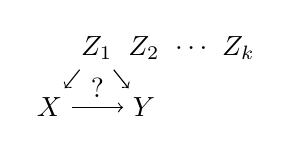
\begin{tikzpicture}[yscale=.75, xscale=.6]
				\node (x) at (0,0) {$X$};
				\node (y) at (2,0) {$Y$};
				\node (z) at (1,1) {$Z_1$};
				\node at (2,1) {$Z_2$};
				\node at (3,1) {$\ldots$};
				\node at (4,1) {$Z_k$};
				\draw [->] (x) edge node [midway, above] {?} (y);
				\draw [->] (z) -- (y);
				\draw [->] (z) -- (x);
			\end{tikzpicture}
	\end{figure}
\end{frame}

\begin{frame}
	\frametitle{Empirical Analysis: Discrimination}
	\begin{figure}
		\centering
		\includegraphics{imgs/accuracy.pdf}
		\caption*{(a) Accuracy (shading: mean $\pm$ standard error, $N=200$)
		of classifying simulated binary datasets (sample size: $1000$)
		as conditionally dependent or independent. (b) The data generating DAG.}
	\end{figure}

\end{frame}

\begin{frame}
	\frametitle{Epirical Analysis: Discrimination Data Generation (Ordinal)}
	Similar analysis as last one but for ordinal datasets.
\end{frame}

\begin{frame}
	\frametitle{Empirical Analysis: Discrimination (Ordinal)}
	\begin{figure}
		\centering
		\includegraphics{imgs/accuracy_ordinal.pdf}
		\caption*{Accuracy (shading: mean $\pm$ standard error) of
		classifying simulated ordinal data (8 levels per variable) as
		conditionally dependent or independent.}	
	\end{figure}
	\footnotetext[7]{JT = Jonckheere-Terpstra test}
\end{frame}

\begin{frame}
	\frametitle{Applications: Model testing Data generation}
	\begin{itemize}
		\item Given a DAG, how well is the test able to identify all the implied CIs in data simulated from the DAG.
		\item We generate random DAGs with varying edge density to generate implied CIs with varying number of conditional variables.
		\item Test the precision and recall of identify implied CI in the simulated dataset.
	\end{itemize}
\end{frame}

\begin{frame}
	\frametitle{Applications: Model testing}
	\begin{figure}
		\centering
		\includegraphics{imgs/model_testing.pdf}
		\caption*{Precision and recall (shading: mean $\pm$ standard
		error) of testing implied CIs and equal number of randomly
		generated CIs in binary datasets (sample size: $1000$)
		simulated from random DAGs on $ 20 $ variables.}
	\end{figure}
\end{frame}

\begin{frame}
	\frametitle{Constraint-Based Structure Learing}
	\begin{itemize}
		\item Systematically performs CI tests on a given dataset to construct a network structure.
		\item Starts with a fully connected network and removes edges $ X \to Y $ if $ X \ci Y | Z $ in data.
		\item The number of variables in $ Z $ is increased in each iteration.
		\item The algorithm reaches higher number of conditional variables in denser graphs.
	\end{itemize}
\end{frame}

\begin{frame}
	\frametitle{Applications: Structure Learing data generation}
	\begin{itemize}
		\item Test how well is the test able to recover a DAG from data simulated from it.
		\item We vary the edge density while keeping the sample size same.
		\item We compute the F-1 score to test how well is the DAG structure recovered.
	\end{itemize}
\end{frame}

\begin{frame}
	\frametitle{Applications: Structure Learning}
	\begin{figure}
		\centering
		\includegraphics{imgs/sl_density.pdf}
		\caption*{Structure learning on simulated data. F1-score
		(shading: mean $\pm$ standard error) of the learned model
		skeletons for randomly generated DAGs with $20$ variables and
		varying edge probabilities.}
	\end{figure}
\end{frame}

\begin{frame}
	\frametitle{Applications: Structure Learning}
	\begin{figure}
		\centering
		\includegraphics{imgs/sl.pdf}
		\caption*{Structure learning on (a) ``alarm'', and (b)
		``insurance'' datasets.  F1-score (shading: mean $\pm$ standard
		error, $N=10$) of the learned model skeletons.}
	\end{figure}
\end{frame}

\begin{frame}
	\frametitle{Applications: Structure Learning}
	\begin{figure}
		\centering
		\begin{subfigure}{0.5\textwidth}
			\centering
			\includegraphics[scale=0.85]{imgs/sl-adult-rf.pdf}
			\caption*{}
			\label{fig:sl_adult_model}
		\end{subfigure}%
		\begin{subfigure}{0.5\textwidth}
			\centering
			\includegraphics{imgs/adult_F1.pdf}
			\caption*{}
			\label{fig:sl_adult}
		\end{subfigure}
		\caption*{Structure learning on US census income dataset. (a)
		Learnt skeleton using RFT. (b) F1-score (shading: mean $\pm$
		standard error, $N=10$) when comparing $d$-connected variable
		pairs from the CPDAG to correlated variable pairs in the
		dataset.}
	\end{figure}
\end{frame}

\begin{frame}
	\frametitle{Runtime Analysis}
	\begin{figure}
		\centering
		\includegraphics{imgs/runtime.pdf}
		\caption*{Runtime (shading: mean $\pm$ standard error, $N=100$)
		for CI tests with varying numbers of conditional variables and
		$1000$ samples per dataset.
		}
	\end{figure}
\end{frame}

\section{Conclusion}
\begin{frame}
	\frametitle{Conclusion/Future Work}
	\begin{itemize}
		\setlength\itemsep{1em}
		\item A residualization based CI test that works for all combination of data types.
		\item Properties: 1) Simple to implement; 2) Interpretable chi-square test statistic; 3) Symmetric by construction; 4) Computationally feasible
		\item Performs reasonably well for low number of
			conditional variable but performs better for high
			number of conditional variables.
		\item For structure learning, a hybrid approach can be used with other
			tests.
		\item Since Random Forests can work with combination of discrete and 
			continuous variables, can possibly be extended to a single 
			unified test.
	\end{itemize}
\end{frame}

\begin{frame}
	\begin{center}
		\Huge{Thanks for listening} \newline
		\Huge{Questions}
	\end{center}
	\begin{center}
		Paper preprint: https://arxiv.org/pdf/2206.04356.pdf
	\end{center}
\end{frame}

\end{document}
